\chapter{Entwicklung einer klaren Erwartungshaltung}
\label{chap:erwartungshaltung}
Dieses Kapitel befasst sich mit der Methodologie und Durchführung von Experteninterviews mit dem Ziel wichtige Aspekte einer \emph{Bedarfsmeldung} durch eine qualitative Inhaltsanalyse zu identifizieren, um daraus Anforderungen an das zu Entwickelnde System zur Extraktion relevanter Informationen aus semistrukturierten \emph{Bedarfsmeldungen} zu entwickeln.
\section{Experteninterviews}
\label{sec:beschreibung-der-interviews}
Im Rahmen der vorliegenden Ausarbeitung werden halbstrukturierte Interviews mit Experten aus dem Bereich des \emph{Staffings} durchgeführt. Sinn und Zweck von Experteninterviews ist die Rekonstruktion spezifischer Wissensbestände oder besonders exklusiver, detaillierter oder umfassender Kenntnisse über bestimmte Wissensbestände und Praktiken.\\

Der Begriff \emph{Experte} bezeichnet eine Person, die über einen privilegierten Zugang zu Informationen verfügt \cite{pfadenhauer2009eye}. Die Expertise eines Experten ist jedoch nicht allein durch die Informationen definiert, über die er exklusiv verfügt \cite{pfadenhauer2009eye}. Auch die Verantwortung für Problemlösungsentscheidungen ist ein entscheidender Faktor \cite{pfadenhauer2009eye}. Diesbezüglich ist Kompetenz erforderlich, die mit Verantwortung und mit Fähigkeiten sowie mit der Bereitschaft, Verantwortung zu übernehmen, verbunden ist \cite{pfadenhauer2009eye}. Dabei ist zu beachten, dass Verantwortung, Fähigkeiten und Bereitschaft in der Regel zusammenfallen \cite{pfadenhauer2009eye}.\\ 

Die Experteninterviews in dieser Ausarbeitung zielen darauf ab, qualitative Daten zu erheben. Die Interviews werden als Einzelinterviews durchgeführt, wodurch der Fokus auf das spezifische Wissen jedes Befragten gerichtet werden kann. Jeder Interviewpartner reagiert individuell aufgrund seines eigenen Vorwissens auf die Interviewfragen und beeinflusst daher nicht die Aussagen anderer Interviewteilnehmer. Die Ergebnisse der Interviews bilden die Grundlage für die Formulierung der Anforderungen einer optimalen \emph{Bedarfsmeldung}, welche als Basis für das zu entwickelnde System eingesetzt wird. Die Interviews wurden in Teams abgehalten und jedes Interview wird zu Dokumentationszwecken aufgezeichnet. Um die Interviews strukturiert für die qualitative Inhaltsanalyse vorzubereiten, ist es erforderlich sie in schriftliche Transkripte umzuwandeln. Zur ersten Textumwandlung wurde das Transkriptionstool von Teams verwendet. Ungenaue Umwandlungen wurden mit der Videoaufnahme nachgebessert. Grundsätzlich wird die einfache Transkribierung nach Dresing und Pehl angewandt \cite{dresing2015praxisbuch}. Im Rahmen dieses Schritts wird der Text vom Umgangssprachlichem in einen gut Lesbaren Text ohne Lücken übersetzt. Der Interviewer wurde mit einem „I“ und die jeweils befragte Person mit „B“ gekennzeichnet. Im Rahmen des Transkriptionsprozesses werden die Aussagen der Interviews anonymisiert. Dies bedeutet, dass personenbezogenen Informationen durch neutrale Bezeichnungen ersetzt werden.\\

Im Vorfeld der Durchführung der Interviews wurde eine Überprüfung der inhaltlichen Verständlichkeit der Fragen sowie ihrer Beantwortbarkeit vorgenommen. Zudem wurde Feedback zur Reihenfolge der Fragen eingeholt. Zu diesem Zweck wurden die Fragen vorab an eine Führungsperson geschickt und schriftlich beantwortet. Die Fragen wurden den Experten vorab inklusive Kontext des Interviews geschickt, damit diese sich bei Bedarf Gedanken machen können. Zur zeitlichen Begrenzung wird das Interview auf zehn Fragen reduziert. Trotz der vorgegebenen Strukturierung des Interviews wird Raum für spontane Fragen gelassen, um eine natürliche Gesprächsführung zu ermöglichen. Die Fragen dienen als Orientierungshilfe und Leitfaden durch das Interview. Der Leitfaden ist dabei lediglich als inhaltliche Richtlinie zu verstehen, von der situativ abgewichen werden kann.
\section{Ablauf der Interviews}
\label{sec:ablaufexperteninterviews}
Im Rahmen der Interviews erfolgt zunächst eine Einführung in die Problemstellung sowie das Ziel der Ausarbeitung. Auf diese Weise wird sichergestellt, dass die Interviewpartner den Sinn und Zweck des Interviews nachvollziehen können. Des Weiteren erfolgt eine definitorische Erläuterung des Begriffs \emph{Bedarfsmeldung}. Auch wenn dies die fachliche Bezeichnung darstellt, ist sie nicht jedem einzelnen Experten geläufig. Im Rahmen der Einführung erfolgt zunächst eine Erörterung der Rolle des Experten bei \emph{adesso}. Im Rahmen dessen erfolgt eine Klärung der genauen Aufgaben des Experten bei \emph{adesso}. Im Anschluss erfolgt eine Erörterung der Rolle des Experten im Kontext des \emph{Staffing}-Prozesses sowie der Bearbeitung der \emph{Bedarfsmeldung}. Die Interviewfragen sind so konzipiert, dass sie zunächst allgemein gehalten sind und im Verlauf des Interviews zunehmend präziser werden. Im Anschluss an die Erörterung der Frage, welche Art von Projekten über \emph{Bedarfsmeldungen} erfasst wird, wird die Frage aufgeworfen, auf welche Weise diese kommuniziert und dokumentiert werden. Im Anschluss erfolgt eine Klärung der für die Erfassung von \emph{Bedarfsmeldungen} relevanten Informationen. Dabei wird erörtert, welche Informationen von besonderer Bedeutung sind und folglich nicht fehlen dürfen. Die Herausforderungen und Bewertungskriterien geben Aufschluss über die bereits genutzten Ansätze zur Standardisierung der \emph{Bedarfsmeldungen}. Des Weiteren können bereits unternommene Maßnahmen zur Qualitätssicherung als hilfreicher Ansatz zur Identifizierung von Anforderungen der \emph{Bedarfsmeldungen} herangezogen werden. Die Beantwortung der Fragen erfordert insbesondere die Entwicklung eigener Ideen und Konzepte, die im weiteren Verlauf des Prozesses zur Erfassung von \emph{Bedarfsmeldung} gegebenenfalls noch nicht zum Einsatz gekommen sind.
\section{Übersicht der Experten}
\label{sec:experten}
Die Übersicht der interviewten Experten ist in der Tabelle \ref{tab:experten} aufgeführt.
\begin{center}
	\begin{tabularx}{1\textwidth} { 
			| >{\raggedright\arraybackslash}X 
			| >{\raggedright\arraybackslash}X
			| >{\raggedright\arraybackslash}X
			| >{\raggedright\arraybackslash}X
			| >{\raggedright\arraybackslash}X | }
		\hline
		Nr. und Datum
		& Profil der Befragten & Durchführungs-art & Dauer & Transkripte (Anhang)\\
		\hline
		\hline
		1. 28.03.2024 & CC-Leiter und Softwarearchitekt & schriftlicher Vorabtest & - & \ref{interview1}\\
		\hline
		2. 29.04.2024 & CC-Leiter und Projektleiter & Video-Interview & 15min & \ref{interview2}\\
		\hline
		3. 29.04.2024 & CC-Leiter und Delivery Manager & Video-Interview & 45min & \ref{interview3}\\
		\hline
		4. 30.04.2024 & CC-Leiter und Softwarearchitekt & Video-Interview & 15min & \ref{interview4}\\
		\hline
		5. 6.05.2024 & Bereichsleiter & Video-Interview & 25min & \ref{interview5}\\
		\hline
	\end{tabularx}\\
	\captionof{table}{Übersicht der Experten}
	\label{tab:experten}
\end{center}
Die erste Spalte der Tabelle \ref{tab:experten} zeigt die vergebene Nummerierung sowie das Datum der Durchführung. Dies dient der vereinfachten Referenzierung innerhalb der nachfolgenden Analyse. Die zweite Spalte der Tabelle enthält die Rolle bzw. Tätigkeit der Befragten bei \emph{adesso}. Alle Befragten haben, oder hatten eine Leitende Rolle mit Erfahrungen in der Personaleinsatzplanung. Dementsprechend hat jeder Befragte in irgend einer Form Berührungspunkte mit Bedarfsmeldungen gehabt. Interview 2 und 3 haben zusätzlich noch die Perspektive zur Erstellung und Verwaltung von Bedarfsmeldungen, da ihre Hauptaufgaben genau in diesem Bereich Fallen. Die 3. Spalte zeigt die Art der Befragung. Abgesehen von dem Vorabtest wurden alle Interviews in einem Video-Call abgehalten. Die vierte Spalte zeigt die Dauer der Interviews. Die letzte Spalte ist eine Referenzierung zu den Transkripten der Interviews im Anhang.\\

Die erste Befragte Person aus dem schriftlichen Vorabtest ist studierter Informatiker mit Diplomabschluss. Bei \emph{adesso} nimmt er die Rolle des CC-Leiters ein. Dies ist die Bezeichnung für Führungspersonen mit Zuständigkeiten für Mitarbeiter bei \emph{adesso}. CC-Leiter haben mit Bedarfsmeldungen zu tun, da sie ihre eigenen Mitarbeiter auf Projekte einstellen müssen. Neben der Tätigkeit als Führungsperson ist er Softwarearchitekt und leitet teilweise Projekte.\\

Die zweite befragte Person hat eine Ausbildung zum Fachinformatiker für Anwendungsentwicklung in einem Softwarehaus abgeschlossen. 7 Jahren Erfahrungen als Consultant wurde er innerhalb von 12 Jahren vom Softwareentwickler zum IT-Leiter einer mittelständigen Bank. Nun ist er als CC-Leiter und Projektleiter bei \emph{adesso} tätig.\\

Die dritte befragte Person war während seiner Laufbahn bei \emph{adesso} als CC-Leiter tätig. Aktuell ist er in einer Mischform von Projektleitung und Produktunterschiede um interne Projekte. Zudem übernimmt er auch noch die Rolle des Delivery Managers, bei dem er eine Schnittstellenposition zwischen \emph{adesso} und den Kunden einnimmt. Dabei geht es unter anderem auch um die Verwaltung der \emph{Bedarfsmeldungen}.\\

Die vierte Befragte Person ist Studierter Kerninformatiker mit einem Diplomabschluss. 2003 startete die Karriere als Sotfware Entwickler und seitdem ist er Software Architekt und CC-Leiter bei \emph{adesso}.\\

Die fünfte Person ist studierter Informatiker mit einem Diplomabschluss. Mit Umwegen ist er im Bereich der Dienstleistung gewechselt. Bei \emph{adesso} ist er CC-Leiter und Bereichsleiter. Er übernimmt das Kunden Management und ist für die Gemeinsame Gestaltung der Zusammenarbeit mit Kunden, aber nicht so sehr für einzelne Bedarfsmeldungen zuständig.\\




%Zur Beantwortung der Forschungsfragen 2 und 3 dieser Arbeit werden
%Experteninterviews mit E-Learning Experten durchgeführt. Nachdem für die
%Beantwortung der Forschungsfrage eins bereits auf die Theorie eingegangen wurde, soll
%nun diese durch praktische Erfahrungen ergänzt werden. In Forschungsfrage 2 werden
%die Anforderungen der Praktiker an einen kultursensitiven Leitfaden herausgearbeitet.
%Um diese Anforderungen angemessen herauszuarbeiten ist eine ausführliche
%Vorbereitung notwendig. Diese Vorbereitung wird in diesem Kapitel erläutert. Zu
%Beginn dieses Kapitels wird allgemein auf die qualitative Forschung eingegangen und
%im Anschluss daran auf die Vorbereitung der Interviews sowie die Vorgehensweise bei
%der Durchführung der Interviews. Das Kapitel schließt mit einer kurzen Einordnung der
%Interviewpartner, bezüglich Haupttätigkeitsfeld im E-Learning und der
%Mitarbeiteranzahl des Unternehmens, ab. 


%Methodik erklären, siehe Wirtschaftsinformatik Bachelorarbeit (S.34)
%genau die Schritte der Fragen erklären. Warum diese Reihenfolge

%nochmal eine bedarfsmeldung genau erklären und die schritte wie bedarfsmeldung erhalten, gepflegt etc wird erklären

%\begin{enumerate}
%	\item Welche Art von Projekten sind typischerweise in Ihrem Unternehmen an der Tagesordnung? Können Sie uns Beispiele für verschiedene Arten von Projekten geben, die \emph{adesso} durchführt?
%	\item Wie werden Projektbedarfe und -anforderungen innerhalb von \emph{adesso} typischerweise kommuniziert und dokumentiert?
%	\item Welche Informationen halten Sie in einer Bedarfsmeldung für besonders wichtig oder unverzichtbar?
%	\item Wie detailliert sollten Projektbeschreibungen Ihrer Meinung nach sein? Sind bestimmte Schlüsselaspekte oder -informationen in jeder Bedarfsmeldung enthalten?
%	\item Welche Herausforderungen oder Schwierigkeiten sind bei unklaren oder unvollständigen Bedarfsmeldungen aufgetreten?
%	\item Wer sind die typischen Stakeholder bei der Erstellung von Bedarfsmeldungen und welche Rolle spielen sie?
%	\item Wie wird die Qualität von Bedarfsmeldungen bei \emph{adesso} bewertet? Gibt es bestimmte Kriterien oder Standards, anhand derer Bedarfsmeldungen beurteilt werden?
%	\item Wie können Sie die Qualität und Klarheit von Bedarfsmeldungen verbessern?
%	\item Welche Auswirkungen haben unklare oder fehlende Informationen in Bedarfsmeldungen auf die Effizienz und den Erfolg von Projekten?
%	\item Wie können Sie sicherstellen, dass die Bedürfnisse und Anforderungen aller relevanten Stakeholder in einer Bedarfsmeldung angemessen berücksichtigt werden?
%\end{enumerate}

\section{Auswertungsmethode}
Zur systematischen Analyse der Experteninterviews wurde die qualitative Inhaltsanalyse nach Philipp Mayring angewendet. Das Ziel der Inhaltsanalyse ist die Zusammentragung der Informationen aus den Interviews. Grundsätzlich unterscheidet sich die Inahltsanalyse in drei Grundtechniken: (i)\emph{Zusammenfassung} (Materialreduktion, um die wesentlichen Inhalte zu erhalten), (ii)\emph{Explikation} (Verständniserweiterung durch Herantragung von Zusatzmaterial) und (iii)\emph{Strukturierung} (Herausfilterung von Aspekten und Einschätzung von Kriterien) \cite{mayring1994qualitative}.\\

Im Folgenden wird sich auf die Technik der Zusammenfassung konzentriert, da die Anforderungen an \emph{Bedarfsmeldungen} nur durch eine Übersicht der Interviewergebnisse erstellt werden kann.\\

Zur strukturierten Analyse werden die Arbeitsschritte mit Hilfe des Ablaufmodells von Mayring aufgeteilt, das in der Abbildung \ref{fig:ablaufmodell} dargestellt ist.
\begin{figure}[H]%htb
	\centering  
	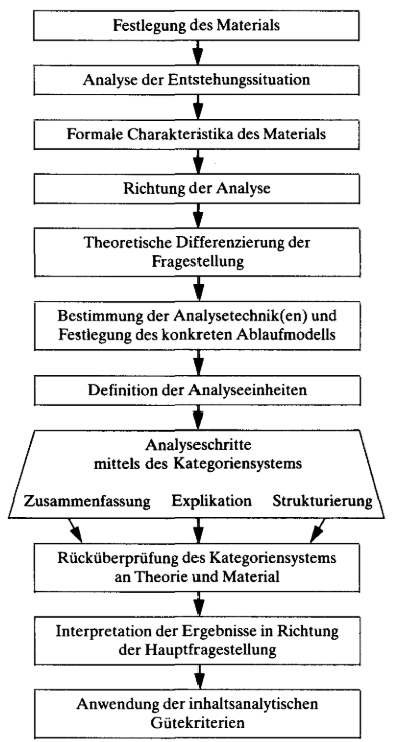
\includegraphics[scale=1]{Abbildungen/Ablaufmodell.png}
	\caption{Allgemeines Ablaufmodell qualitativer Inhaltsanalyse (Mayring, 1988) \cite{mayring2019qualitative}}
	\label{fig:ablaufmodell}
\end{figure}\mbox{} \\
Diese Struktur des allgemeinen Ablaufmodells wird Schrittweise auf die Interviews angewendet.
\paragraph{Festlegung des Materials}\mbox{} \\
Die Materialien sind aus 4 Experteninterviews und einem schriftlichen Vorabtest entnommen worden. Dazu wurden 10 Interviewfragen als Leitfaden angewendet.
\paragraph{Analyse der Entstehungssituation}\mbox{} \\
Die Interviewteilnehmer sind Führungskräfte, die bereits mit \emph{Bedarfsmeldungen} Berührungspunkte hatten. Vereinzelt haben diese auch näheren Kontakt mit \emph{Bedarfsmeldungen}. Dies ist in Kapitel \ref{sec:experten} näher erläutert.
\paragraph{Formale Charakteristika des Materials}\mbox{} \\
Die Interviews wurden über Teams mit der Aufnahmefunktion aufgezeichnet und mit der Teams Transkriptionsfunktion transkribiert. Undeutliche Transkriptionsbereiche wurden mit der Aufnahme nachgebessert. Dementsprechend liegen die Interviews in Textform im Anhang zur Verfügung.
\paragraph{Richtung der Analyse}\mbox{} \\
Das Ziel der Analyse ist die Informationsgewinnung aus den Interviews, um die wichtigsten Aspekte von \emph{Bedarfsmeldungen} zu identifizieren. Dabei soll der Fokus auf den Inhalt gelegt werden, wodurch emotionale und sprachliche Faktoren nicht einbezogen werden.
\paragraph{Theoretische Differenzierung der Fragestellung}\mbox{} \\
Die Interviews sind auf die Aussagen der Experten aus Teilbereichen der Fachkräfteorganisation und der Akquirierung und Bearbeitung von Projekten und Projektbedarfen zugeschnitten. Es geht um den Informationsgehalt von \emph{Bedarfsmeldungen}. Dafür wurden Themenfelder festgelegt, die Aussagen über die Relevanz und Konsistenz der \emph{Bedarfsmeldungen} sein können. Der Ablauf und die dazugehörigen Themenfelder wurden bereits in Kapitel \ref{sec:ablaufexperteninterviews} erläutert und spiegeln sich in den Fragen wider.
\paragraph{Bestimmung der Analysetechnik und Festlegung des konkreten Ablaufmodells}\mbox{} \\
Zur Extraktion der relevanten Informationen wurde die zusammenfassende Inhaltsanalyse nach Mayring verwendet. Innerhalb der Analyse wird der Text auf wesentliche Inhalte reduziert und in Kategorien unterteilt. Die einzelnen Schritte des Ablaufmodells für eine zusammenfassende Inhaltsanalyse ist in Abbildung \ref{fig:zusammenfassendeinhaltsanalyse} abgebildet.
%\begin{figure}[H]%htb
%	\centering  
%	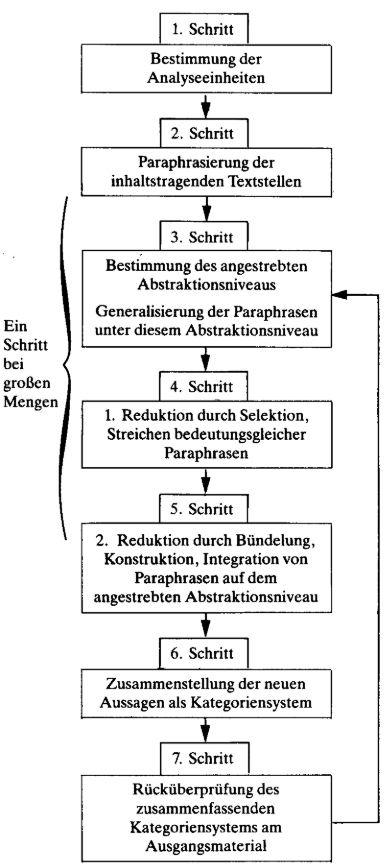
\includegraphics[scale=0.5]{Abbildungen/zusammenfassendeInhaltsanalyse.png}
%	\caption{Ablaufmodell zusammenfassender Inhaltsanalyse (Mayring, 1988) \cite{mayring2019qualitative}}
%	\label{fig:zusammenfassendeinhaltsanalyse}
%\end{figure}\mbox{} \\

\begin{figure}[H]
	\begin{minipage}[b]{.4\linewidth} % [b] => Ausrichtung an \caption
		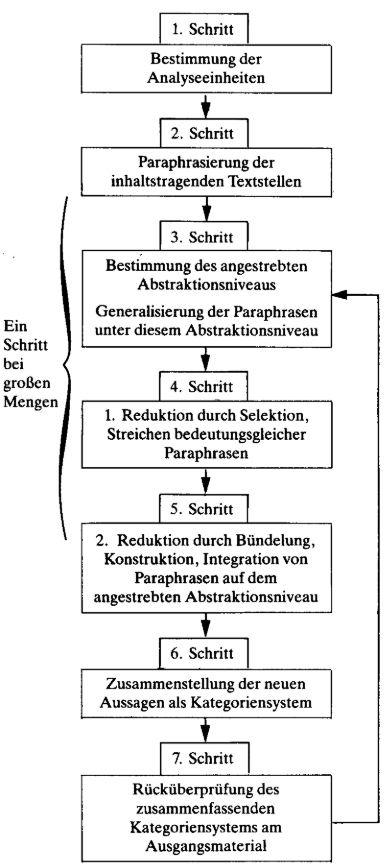
\includegraphics[scale=0.5]{Abbildungen/zusammenfassendeInhaltsanalyse.png}
		\caption{Ablaufmodell zusammenfassender Inhaltsanalyse (Mayring, 1988) \cite{mayring2019qualitative}}
		\label{fig:zusammenfassendeinhaltsanalyse}
	\end{minipage}
	\hspace{.1\linewidth}% Abstand zwischen Bilder
	\begin{minipage}[b]{.4\linewidth} % [b] => Ausrichtung an \caption
		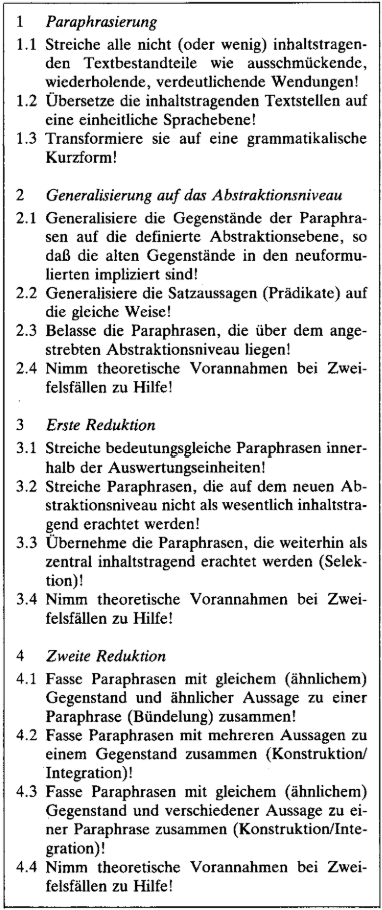
\includegraphics[scale=1]{Abbildungen/verfahrensregeln.png}
		\caption{Verfahrensregeln zusammenfassender Inhaltsanalyse (Mayring, 1988) \cite{mayring2019qualitative}}
		\label{fig:verfahrensregeln}
	\end{minipage}
\end{figure}
Die Interviews werden auf die wichtigsten Informationen reduziert und mit Berücksichtigung der Verfahrensregeln aus der Abbildung \ref{fig:verfahrensregeln} paraphrasiert. Die Verfahrensregeln beschreiben Arbeitsschritte bei der Durchführung der zusammenfassenden Inhaltsanalyse.
\paragraph{Bestimmung der Analyseeinheiten}\mbox{} \\
Mayring beschreibt drei Analyseeinheiten. Die (i)\emph{Auswertungseinheit} definiert, welche Textteile jeweils nacheinander kodiert werden \cite{mayring1994qualitative}. Die (ii)\emph{Kodiereinheit} definiert, welche minimale Materialmenge ausgewertet werden darf und welcher Kategorie sie zugeordnet werden kann \cite{mayring1994qualitative}. Die (iii)\emph{Kontexteinheit} definiert die maximale Textmenge, die unter eine Kategorie fallen kann \cite{mayring1994qualitative}.
\todo{beschreiben wie ich das gemacht habe}
%\paragraph{Interview Zusammenfassung}\mbox{} \\
%\todo{ich glaube ich brauche diesen Abschnitt nicht...}\\
%In diesem Abschnitt werden die Schritte 2 bis 5 aus dem Ablaufmodell der Abbildung \ref{fig:zusammenfassendeinhaltsanalyse} durchgeführt. Dabei werden alle Interviews heruntergebrochen und paraphrasiert. Die Schritte werden aufgrund der Menge an Materialien in einem Schritt dargestellt.
%\begin{enumerate}
%	\item Wer sind die typischen Stakeholder bei der Erstellung von Bedarfsmeldungen und welche
%	Rolle spielen sie?\\
%	
%	-1. Experte Sales/PL: Anforderer mit den technischen Informationen, Maitre: kümmert sich um das Staffing bzw. die eigentliche Besetzung
%	-Stakeholder sind klassisch die Fachverantwortlichen beim Kunden, aber auch die Entscheider. Sprich also deren Vorgesetzte die quasi fachlich vielleicht das ganze nicht so bewerten können, aber das Budget dafür hergeben müssen und natürlich dann im Zweifelsfall auch CO, CEO oder sogar Geschäftsführer
%	-Kunde, Delivery Manager, als Projektleiter, als Programm Manager, als Account Manager oder Vertriebler mit Kunden sprechen, in Projekte reinschauen, Projektorganisationen definieren und selbst in diesen Rollen eine Bedarfsmeldung erfassen
%	-für die Erstellung der Bedarfsmeldungen der Projektleiter und Maitre eigentlich relevant
%	-Sales oder der interne Maitre dafür zuständig ist, stellt quasi eine Bedarfsmeldung im Normalfall auf Basis von Anforderungen direkt vom Kunden, Oder es kommt konkret im Projekt aus mündlich genannten Bedarfsmeldungen. Das kann auch durch ein Scrum Master oder Product Owner entsprechend entstehen. Da ist dann derjenige, der die Bedarfsmeldung erstellt auch zuständig
%	\item Welche Art von Projekten sind typischerweise in Ihrem Unternehmen an der Tagesordnung?
%	Können Sie uns Beispiele für verschiedene Arten von Projekten geben, die adesso
%	durchführt?\\
%	
%	-Software-Entwicklungsprojekte, angefangen von Projekten in dem ein adessi in einem Kundenprojekt arbeitet über gemischte Teams aus adessi und Kunde bis hin zur kompletten Lieferung von %Projekleitern, Testern, Requirements Engineer und Entwicklern
%	-2 Arten von Projekten teilen. Aus einer sind Time Material Projekte, wo quasi der Kunde mit einer Idee kommt, wo wir gut unterstützen können, Festpreis Projekten haben wir eher die Staffing Hoheit. Das heißt, wir können entscheiden wen wir in das Projekt einsetzen
%	-gibt Projekte, die ein Kunde eine Kundenorganisation aufsetzt und durchführt, an denen wir uns dann beteiligen, indem wir beispielsweise in bestimmte Rollen an bestimmte Stellen dort Menschen reinbringen, Das andere ist, wenn wir im Kundenauftrag Projekte aufsetzen --> Projekte unter unserer Kontrolle im Kundenauftrag und dann gibt es natürlich auch interne Projekte, Consulting
%	-über das Jira erfasst und entsprechend auch mit allen beteiligten Parteien geteilt
%	-demjenigen der es einstellt, werden die Kriterien definiert und in einem JIRA-Ticket überführt --> Felder, die strukturiert sind. Z.B zu welchem Tagessatz das ganze angeboten wird, wann das Ganze startet, wie hoch das Volumen also an Tagen ist. Es gibt einige Freitextfelder, bei dem drinsteht, was die Aufgaben usw. sind. Zum Beispiel bei einer Rahmenvereinbarung, die wir gerade machen gibt es dann ein Excel, was ausgefüllt werden muss mit seiner Selbstbeurteilung, nutzen wir doch JIRA, weil es im Normalfall nicht genau den einen Case gibt, wie wir Bedarfsmeldung reinkriegen
%	
%	TEXT
%	\item Wie werden Projektbedarfe und -anforderungen innerhalb von adesso typischerweise
%	kommuniziert und dokumentiert?\\
%	
%	-Initial über den Maitre, der das Staffing übernimmt bzw. auch Vorschläge von Projektleitenden zum Staffing annimt, teilweise auch über das eigene Netzwerk zwischen Führungskräften, im CC, Bereich oder der LoB. Am Ende über das Staffing Jira
%	-
%	
%	TEXT
%	\item Welche Informationen halten Sie in einer Bedarfsmeldung für besonders wichtig oder
%	unverzichtbar?\\
%
%	TEXT
%	\item Wie detailliert sollten Projektbeschreibungen Ihrer Meinung nach sein? Sind bestimmte
%	Schlüsselaspekte oder -informationen in jeder Bedarfsmeldung enthalten?\\
%	
%	TEXT
%	\item Wie wird die Qualität von Bedarfsmeldungen bei adesso bewertet? Gibt es bestimmte
%	Kriterien oder Standards, anhand derer Bedarfsmeldungen beurteilt werden?\\
%	
%	TEXT
%	\item Wie können Sie die Qualität und Klarheit von Bedarfsmeldungen verbessern?\\
%	
%	TEXT
%	\item Welche Herausforderungen oder Schwierigkeiten sind bei unklaren oder unvollständigen
%	Bedarfsmeldungen aufgetreten?\\
%	
%	TEXT
%	\item Welche Auswirkungen haben unklare oder fehlende Informationen in Bedarfsmeldungen
%	auf die Effizienz und den Erfolg von Projekten?\\
%	
%	TEXT
%	\item Wie können Sie sicherstellen, dass die Bedürfnisse und Anforderungen aller relevanten
%	Stakeholder in einer Bedarfsmeldung angemessen berücksichtigt werden?\\
%	
%	TEXT
%\end{enumerate}
\paragraph{Zusammenstellung der Aussagen als Kategoriesystem}\mbox{} \\
Die Kategorien sind induktiv aus dem Material erstellt worden \cite{mayring2012qualitative}. Die Ergebnisse der Schritte aus dem Ablaufmodell der Abbildung \ref{fig:zusammenfassendeinhaltsanalyse} sind im Anhang \ref{sec:reduktion} in der Tabelle \ref{tab:kategorien} dargestellt. Dabei wurden alle Interviews heruntergebrochen, paraphrasiert, reduziert und in Kategorien (K1-K7) überführt.\\

Nachfolgend sind die Ergebnisse aus der qualitativen Inhaltsanalyse:
\begin{itemize}
	\item[K1] Arten von Projekten
	\begin{itemize}
		\item[-] Kundenprojekte
		\item[-] Softwareentwicklungsprojekte
		\item[-] Time Material
		\item[-] Festpreis
	\end{itemize}
	\item[K2] Stakeholder
	\begin{itemize}
		\item[-] Maitre
		\item[-] Führungskräftenetzwerk
		\item[-] Sales
		\item[-] Projektleiter
		\item[-] Fachverantwortliche
		\item[-] Entscheider
		\item[-] Geschäftsführer
		\item[-] Delivery Manager
		\item[-] Account Manager
	\end{itemize}
	\item[K3] Wichtige Informationen
	\begin{itemize}
		\item[-] Tagessatz
		\item[-] Einsatz
		\item[-] Dauer
		\item[-] Tech Stack
		\item[-] Muss/Kann Kriterien
		\item[-] Einarbeitungszeiträume
		\item[-] Lieferverpflichtung
	\end{itemize}
	\item[K4] Bedarfsmeldung
	\begin{itemize}
		\item[-] Überschrift
		\item[-] Beschreibung
		\item[-] Einsatzkontext
		\item[-] Datum
		\item[-] Volumen
		\item[-] in Jira gespeichert
		\item[-] gewichtete Fähigkeiten
		\item[-] keine feste Struktur
	\end{itemize}
	\item[K5] Qualitätsbewertung
	\begin{itemize}
		\item[-] keine vorhanden
		\item[-] Erfahrung
		\item[-] über Projektleitung
		\item[-] intensives Lesen
		\item[-] Rückfragen stellen
		\item[-] grober Rahmen durch Jira
		\item[-] regelmäßige Meetings
	\end{itemize}
	\item[K6] Qualitätsverbesserung
	\begin{itemize}
		\item[-] klare Vorgaben
		\item[-] weniger Freitext
		\item[-] Reviewprozess
		\item[-] Verständnisübereinstimmung
		\item[-] Beseitigung Missverständnisse
		\item[-] strukturierte Datenerfassung
		\item[-] KI-gestützte Prüfungen
	\end{itemize}
	\item[K7] Auswirkungen
	\begin{itemize}
		\item[-] Überblick verlieren
		\item[-] längerer Staffing-Prozess
		\item[-] Umbesetzung
		\item[-] erhöhter Aufwand
		\item[-] Mehrfachbeantwortung
		\item[-] Missverständnis
		\item[-] unpassendes Personal
	\end{itemize}
\end{itemize}
\section{Interpretation der Ergebnisse}
\todo{was ziehe ich hier für ein Ergebnis raus}\\
Die Kategorien zeigen, dass \emph{Bedarfsmeldungen} Bestandteil eines komplexen und vielschichtigen Prozesses sind, der verschiedene Arten von Projekten, eine Vielzahl von Stakeholdern und detaillierte Informationen umfasst. Die Qualität der Bedarfsmeldungen ist entscheidend für den Erfolg der Projekte, und es existieren Möglichkeiten zur Verbesserung durch Strukturierung, Automatisierung und klarer Kommunikationswege. Die Auswirkungen von unzureichender Pflege und fehlendem Informationsgehalt der \emph{Bedarfsmeldungen} sind weitreichend und können zu erheblicher Ineffizienz und Problemen innerhalb von \emph{adesso} führen.\\

Eine \emph{Bedarfsmeldung} bezeichnet eine Projektbeschreibung, die Anforderungen an ein zu entwickelndes System enthält. Sie umfasst mehrere wesentliche Aspekte, die dafür sorgen klar und effektiv zu sein. Dazu gehört eine Überschrift, die die Projektart und den Bedarf kurz zusammenfasst. Die Beschreibung spiegelt den Bedarf wider und durch den Einsatzkontext können wichtige Hintergrundinformationen zum Umfeld des Projekts erklärt werden. Das Datum gibt Aufschluss über den Zeitplan, in welchem das Projekt durchgeführt werden soll. Durch das Volumen können benötigte Ressourcen und den Umfang des Bedarfs dokumentiert werden. Die \emph{Bedarfsmeldungen} werden in Jira gespeichert und erhalten dadurch einen groben Rahmen, wie diese gepflegt werden. Dennoch existiert keine einheitliche Strukturierung. Dadurch entstehen Abschnitte mit unstrukturiertem Informationsgehalt. Die Informationen sind insofern unstrukturiert, als dass sie ohne vordefinierte Struktur in Form eines Volltexts vorliegen. Infolgedessen kann es zu Abweichungen hinsichtlich der Ausgestaltung von \emph{Bedarfsmeldungen} kommen.\\

Eine \emph{Bedarfsmeldung} sollte den Tagessatz sowie den Einsatzbereich klar definieren. Zudem ist es wichtig, die Dauer des Einsatzes und den Technologie-Stack anzugeben, der zum Einsatz kommt. Darüber hinaus sollten die Muss- und Kann-Kriterien für die gesuchten Fachkräfte klar formuliert werden. Einarbeitungszeiträume und Lieferverpflichtungen sind ebenfalls entscheidende Bestandteile, die in einer \emph{Bedarfsmeldung} nicht fehlen dürfen.

\section{keine Ahnung wie ich es nenne}
\todo{richtig benennen}\\
Die Problemstellung umfasst eine Reihe von Punkten, die im Rahmen der Ausarbeitung zu behandeln sind. Aufgrund der unstrukturierten und mit fehlenden Informationen versehenen \emph{Bedarfsmeldungen} ist eine Standardisierung von besonderer Relevanz. Dies würde die Extraktion relevanter Informationen erleichtern und somit die Effizienz des Systems verbessern. Zudem würde ein solcher Ansatz einen Einblick in die Relevanz von Informationen und Stichpunkten geben. Im Rahmen der weiteren Bearbeitung einer Standardisierung ist die Extraktion der erforderlichen Informationen aus dem Volltext erforderlich. In diesem Kontext existiert bereits eine Reihe an Methoden und Ansätzen, die sich in der Forschung bewährt haben. Der unstrukturierte Volltext muss in eine strukturierte inhaltliche Aufteilung in einzelne Sequenzen und Stichpunkte überführt werden.\\




%\cite{maguire2002user}

%im anhang sind die transskripte
%wenn man nicht ne größere anzahl an infos hat gucken ob man das halb automatisch evaluieren. Vielleicht kategorisieren. Infos die wichtig sind gucken ob die %dann auch nach dem preprocessing drin sind. Regressive tests schreiben.

%transformation von bedarfsmeldung zu guter bedarfsmeldung, was ist der fokus von der bedarfsmeldung, wie gut machen die ansätze das, und muss man das dann noch weiter verarbeiten, haben wir alles was wir brauchen mit nur einem algorithmus, inferenz falls parameter fehlt, gibt es einen der alles löst

%Fragen in das proposal aufnehmen, führungskraft vorher fragen ob die fragen nice sind.
